\documentclass[../main.tex]{subfiles}
\graphicspath{{\subfix{../imagenes/}}}

\begin{document}

\chapter{Conclusions} \label{chap:conclusions} 

    \vspace{-0.2cm}


    The ideas presented in this thesis were driven by the interest and developing more efficient intelligent systems that can adapt to the changing nature of the data they are trained on and research about the problems that arise when trying to achieve this goal and how they can be addressed in a machine learning context.
    
    We applied these concepts to the real-world problem of detecting tuberculosis from sputum smear microscopy images, a task that is challenging due to the scarcity (and reliability) of data available for training and the high cost of annotating data samples. 
    
    \vspace{-0.3cm}
    \section{Summary of Results} \label{conclusions:summary}
    \vspace{-0.3cm}

    Within this context, we can summarize the main contributions of this thesis as follows:
    \vspace{-0.1cm}

    \begin{itemize}
        \item We developed a web-based platform for the annotation of sputum smear microscopy images, which includes a frontend for annotators to label images and a backend for storing and managing the annotations. The platform allows its users to interact with ML models available in the system and use them to assist in the annotation process.
        \item Furthermore, we formalized all the components of this platform, making it easy to extend and adapt to other tasks and problems. We put special interest into understanding the design principles that we can draw from the self-adaptive systems literature and how we could apply them to the design of our platform.
        \item We took a transformer-based neural network model, initially trained on a large-scale dataset of images for object detection, and applied domain adaptation techniques to fine-tune it to the task of detecting tuberculosis from sputum smear microscopy images. This model achieved a high predictable performance compared to baseline models trained for the same task.
        \item We implemented an active learning framework that uses the model's uncertainty to select the most informative samples for annotation, which we used to train the model with a fraction of the data that would otherwise be required to train it from scratch and achieved performance comparable to one trained with 40\% more data.
    \end{itemize}

    Furthermore, we make a thorough review of the state-of-the-art in the fields of computer vision, continual learning, active learning, and domain adaptation, among other machine-learning-related topics, to provide a solid theoretical foundation for the ideas presented in this thesis. We focus our review on how these concepts can be applied to healthcare issues and the specific challenges that arise when doing so.


    \section{Objectives Achieved
        } \label{conclusions:objectives_achieved} 

    Through our experimental setup, we were able to assess how well a continual learning process can improve the performance of an ML model over time and do so while paying attention to how samples should be more efficiently collected (among other aspects). Our results directly demonstrate the adaptive capabilities of the system proposed, showing its ability to mature and refine the performance or models in response to new data.

     By demonstrating the effectiveness of these tactics, we consider that we have achieved our main goal of devising a reliable and self-improving system capable of continuously enhancing the performance of ML models for real and impactful use cases, maximizing its usefulness to methods for the detection of tuberculosis.
     


    \section{Limitations of the System} \label{conclusions:limitations} 

    The main obvious limitation of our system comes directly from our experimental results, which show how active learning can be a double sword when it comes to continually fine-tuning a model using a static pool of data. In each training round (after the most important samples have been identified), the model is fine-tuned with progressively less informative samples, which can lead to a decrease in performance over time (as we observed in our experiments).

    With the random sampling approach, one can expect a more consistent increase in performance as the model is trained with more data since the model is likely being exposed to a more diverse set of samples that are not necessarily the most - or least - important ones for the model to learn from, however, this tactic will be less sample efficient than the active learning approach.
    \clearpage
    Thus, perhaps more of a hybrid approach is needed, where the model is trained with a combination of random and actively sampled data, which is something we did not have time to explore in this thesis.

    Another limitation of the system we identified, especially within the context of this project, is the lack of explainability of the methods we used. While we can show improvements in performance metrics compare them to other models, and get an idea of why certain samples are better for training, it is very difficult to explain the model's behavior in a way that is (1) easy to understand for non-experts and (2) reliable and consistent across different models and datasets, which is a problem when trying to apply them to the healthcare industry.
    
    Methods such as \textit{data attribution}\footnote{Because data attribution has also proven useful for sample selection in active learning, we did some research about the state-of-the-art in this area to see which of them were available and how they could be applied to our system (but did not have time to implement them). Some promising methods are \textit{TRAK} (\cite{park_trak_2023}) and \textit{influence selection} (\cite{liu_influence_2021}).} can be promising in this area of research that can be well applied to the healthcare industry since it allows to trace the contribution of each data sample to the model's predictions, which can be very informative about the model's behavior.
    
    \vspace{-0.3cm}
    \section{Future Work} \label{conclusions:future_work} 
    % \addcontentsline{toc}{section}{Future Work}

    We continue this chapter by discussing some of the most immediate future work that can be done to improve the system we developed and expand on the ideas presented here. 

    \vspace{-0.1cm}
    \subsection{Implementing new adaptation strategies to the system 
    } \label{conclusions:future_work:adaptation_strategies}

    By far, the most interesting future work we envision for the system we developed is to implement new adaptation strategies that can be used to test the continual improvement of ML models. 
    
    In section \ref{sec:continually_adaptive_systems_sota} we introduced concepts like knowledge distillation and adversarial training and formalized how they could be integrated into the system we propose in \ref{sec:formalizing_adaptive_process} but either because of time constraints, resource constraints (e.g., lack of access to a GPU), or simply because it did not fit well with the scope of this thesis, we could not implement or experiment with them in our system.

    However, with the framework we proposed, and the platform we built around it, we consider it should be relatively easy to implement new adaptation strategies and test them. This is the main reason why we put so much effort into formalizing the system and making it easy to extend and adapt to other tasks and problems.

    For these reasons, we consider it to be in the most immediate future in terms of keeping the development of the ideas presented in this work further.

    \subsection{Potential to run the system as a federated learning platform} \label{conclusions:future_work:federated} 

    Another interesting future work direction we envision - which could be enough to be the subject of a whole thesis on its own - is the idea for the system we developed to run as a \textit{federated learning} platform.

    Federated learning is the concept of training a model using data from multiple sources without having to share the data itself. This is achieved by training the model on each source separately and combining the results to obtain a final model. 
    
    Such a system could be based on works like Joshi et al.'s (2022) \cite{joshi_federated_2022}, which demonstrated the benefits of using a federated learning platform to train machine learning models for healthcare uses as a way to protect the privacy of patients and give more utility to the highly-valuable data that is collected in that industry.
    
    As a federated system, the components we proposed in our design would be distributed across multiple clients (or research units), each with its own data. Each client would have its own instance of the platform, which would be connected to a central server that would coordinate the training of the models and the sharing of the trained weights.

    The motivation for this comes from both suggestions made by stakeholders in this project, who expressed interest in the idea of a federated learning system, and personal experience working with healthcare data, where it is challenging to convince partners (even within the same organization) to share their data. 

    Figure \ref{fig:federated} illustrates the concept of a federated learning system:

    \begin{figure}
        \centering
        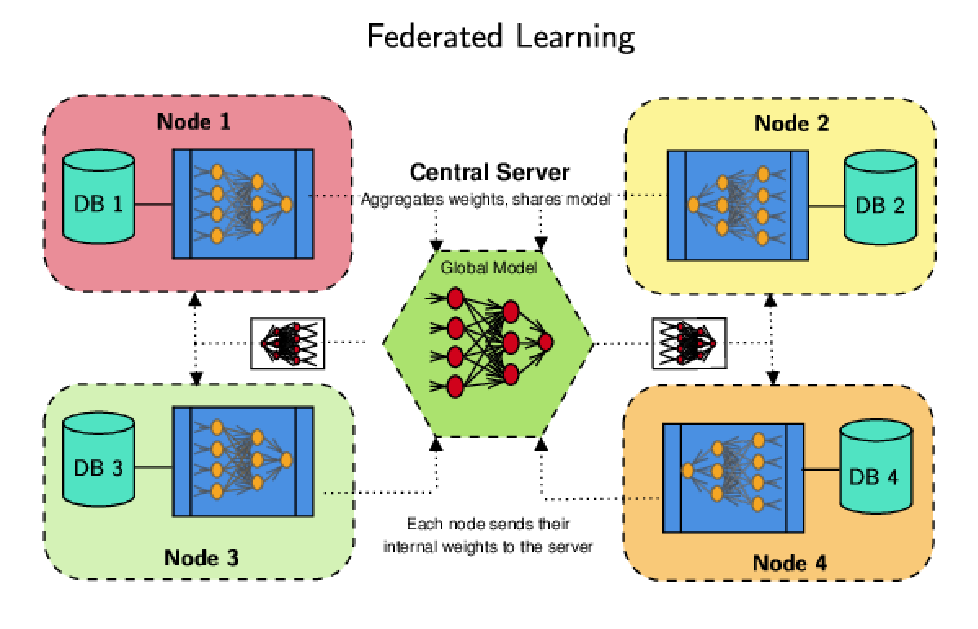
\includegraphics[width=0.85\linewidth]{figures/federated.pdf}
        \caption{Illustration of a Federated Learning System}
        \label{fig:federated}
    \end{figure}


    % \clearpage

    \subsection{Comments on Further Research Directions} \label{conclusions:research_directions}

    In addition to the ideas presented in this section for future work, we also made a relatively lengthy discussion of other topics tangential to the ideas dealt with in this thesis that we consider could be potential for further research. 
    
    Unlike above, where we focused on ways to address limitations of the proposed system or ways to improve it in the immediate future, this discussion takes a broader view, focusing on ideas from emerging fields of research that we consider could be very promising in the future.
    
    As to not distract from the content in this chapter - that is much more relevant to the actual work done -  we present this discussion in the appendix of this thesis (\nameref{appendix:further_research}).
    

    \section{Final Remarks} \label{conclusions:final_remarks} 
    
    Through this thesis, we have presented a system that can be used to continually improve the performance of ML models over time, which we applied to the real-world problem of detecting tuberculosis from sputum smear microscopy images.

    The initial idea to work on the concepts that we presented comes from a personal interest in the field of machine learning and how it can be more efficiently applied to real-world systems. 
    
    Through the development of this thesis, it also came a necessity - and deep interest - to understand the challenges that arise when trying to apply these concepts to the healthcare industry, and the importance that well-designed and reliable systems have in this field.
    
    We consider that the ideas presented in this thesis are a step in the right direction toward achieving this goal, and we hope that they can be useful to other researchers and practitioners in the field. 


    

    % Unlike many scientific advances, breakthroughs such as a true self-improving model that adapts itself continually in an online fashion will have immediate applications in every domain, from healthcare to education, to economics, to scientific discovery itself \dots 

% \printbibliography
\end{document}